\section{Neuronale Netzwerke}

\subsection{Geschichte}

Im Jahr 1943 wurde die erste Arbeit darüber geschrieben, wie Neuronen im Gehirn funktionieren könnten und die Autoren Warren McCulloch und Walter Pitts experimentierten sogar damit diese mit elektronischen Schaltkreisen nachzubauen.\footnote{\cite[]{alogicalcalculus}}

In den 1950er Jahren haben Forscher von IBM daran gearbeitet ein NN\footnote{Kurzform für "`Neuronales Netzwerk"', wird ab jetzt weiterhin verwendet.} mit einem Computer zu simulieren. Der Versuch scheiterte allerdings.\footnote{\cite[Absatz 3]{nnhistory}}

Immer wieder gab es kleinere Forschungsprojekte, ein sehr großer Durchbruch war aber 1975 die Entwicklung eines "`Backpropagation"' Algorithmus durch den Wissenschaftler Paul Werbos. Ähnliche Algorithmen wurden wiederholt und unabhängig entwickelt, aber Werbos' Algorithmus war der erste mit großer Bedeutung.\footnote{\cite[]{paulwerbosbackpropagation}} Das Prinzip des Algorithmus wird auch heute noch verwendet, es ist dieser Algorithmus der dem Neuronalen Netzwerk das selbstständige Lernen ermöglicht.\footnote{Genaueres in Kapitel \ref{funktionsweise}}

In 1998 veröffentlichte Yann LeCun und sein Team eine Arbeit über die Anwendung eines "`Convolutional Neural Networks\footnote{Ab jetzt als CNN bezeichnet}"' zur Erkennung von geschriebenen Zeichen in einem Dokument.\footnote{\cite[]{cnnhistory}} Diese Arbeit gilt als Ursprung des, für beispielsweise Bilderkennungs Software gut geeignete, CNNs und Weiterentwicklungen werden auch heute noch verwendet.

Obwohl ein großes Potenzial erkannt wurde, war es über die nächsten Jahre wieder recht still. Der nächste große Durchbruch passierte in 2012 als Geoffrey Hinton ein Modell entwickelte, was die Fehlerquote in einer öffentlichen Challenge für Bilderkennung beinahe halbierte.\footnote{\cite[]{geoffrey}} Der Grund dafür waren mehrere fundamentale Neuerungen aus dem Bereich Deep Learning; die wahrscheinlich größte Änderung: Starke Parallelisierung des Backpropagation-Prozesses, durch Verschiebung der Last von der CPU auf die GPU. Aufgrund der starken Überlegenheit eines Grafikprozessors in parallelisierten Prozessen, wie die benötigten Tensormultiplikationen durch die deutlich größere Anzahl an (dafür schwächeren) Kernen im Vergleich zu einer herkömmlichen CPU, kann ein NN mehrere hundertmal schneller trainiert werden.

Heute gibt es (vergleichsweise) simple Frameworks, wie das im Jahr 2015 erschienende TensorFlow oder PyTorch aus 2016, welche das erstellen, trainieren und verwenden von NN enorm vereinfachen. Ihr Funktionsumfang wächst durch die große Open-Source Community ständig.

%Sind die Zitate okay?

\begin{figure}[h]
    \begin{chronology}[10]{1940}{2020}{\textwidth}
        \event{1943}{Erste Arbeit und Experimente}
        \event[1950]{1960}{Bemühungen, ein NN digital umzusetzen}
        \event{1975}{Backpropagation Algorithmus}
        \event{1998}{Erfindung des CNNs}
        \event[2015]{2020}{Entwicklung versch. Frameworks}
    \end{chronology}
    \caption[Zeitstrahl]{Zeitstrahl von 1940 bis 2020 mit den wichtigsten Ereignissen der Entwicklung künstlicher Neuronaler Netzwerke}
\end{figure}

\subsection{Aufbau}

\begin{wrapfigure}{r}{10cm}
    
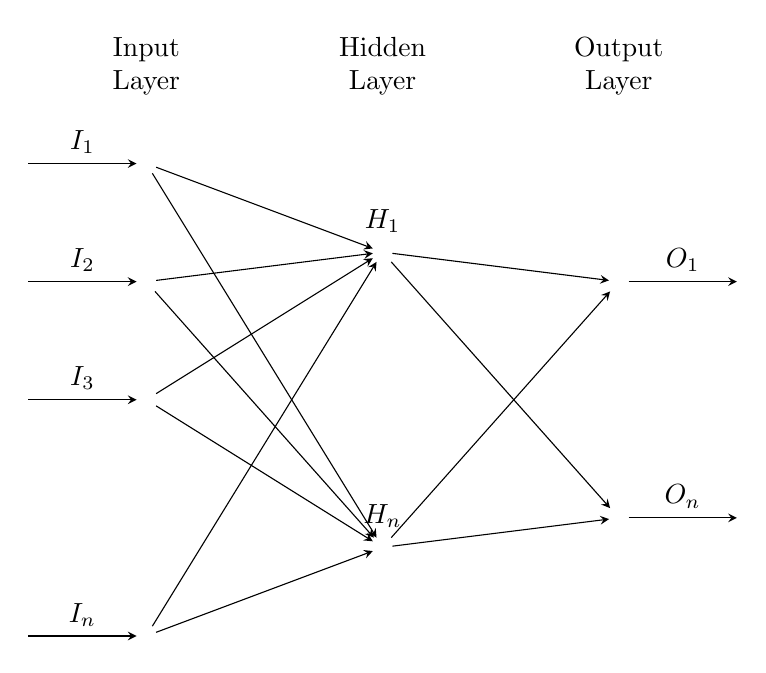
\begin{tikzpicture}[x=1.5cm, y=1.5cm, >=stealth]

    \foreach \m/\l [count=\y] in {1,2,3,missing,4}
    \node [every neuron/.try, neuron \m/.try] (input-\m) at (0,2.5-\y) {};

    \foreach \m [count=\y] in {1,missing,2}
    \node [every neuron/.try, neuron \m/.try ] (hidden-\m) at (2,2-\y*1.25) {};

    \foreach \m [count=\y] in {1,missing,2}
    \node [every neuron/.try, neuron \m/.try ] (output-\m) at (4,1.5-\y) {};

    \foreach \l [count=\i] in {1,2,3,n}
    \draw [<-] (input-\i) -- ++(-1,0)
    node [above, midway] {$I_\l$};

    \foreach \l [count=\i] in {1,n}
    \node [above] at (hidden-\i.north) {$H_\l$};

    \foreach \l [count=\i] in {1,n}
    \draw [->] (output-\i) -- ++(1,0)
    node [above, midway] {$O_\l$};

    \foreach \i in {1,...,4}
    \foreach \j in {1,...,2}
    \draw [->] (input-\i) -- (hidden-\j);

    \foreach \i in {1,...,2}
    \foreach \j in {1,...,2}
    \draw [->] (hidden-\i) -- (output-\j);

    \foreach \l [count=\x from 0] in {Input, Hidden, Output}
    \node [align=center, above] at (\x*2,2) {\l \\ Layer};

\end{tikzpicture}

    \caption[Aufbau]{Vereinfachter Aufbau eines NN}
\end{wrapfigure}

In Abbildung 2 sieht man den Aufbau eines herkömmlichen NN, so wie es noch vor 40 Jahren verwendet wurde. In der Grafik erkennt man drei Layer mit x-beliebigen Neuronen, welche untereinander mit jeweils allen Neuronen der vorigen und nächsten Layer verbunden sind. Die Anzahl der Hidden Layer kann an das Ziel angepasst und  ausgewählt werden und auch die Anzahl der einzelnen Neuronen ist erstmal beliebig, als Faustregel gilt aber:

\begin{itemize}
    \item Die Anzahl der Neuronen in dem Hidden Layer sollte zwischen der Größe des Input und Output Layers liegen.
    \item Die Anzahl der Neuronen in dem Hidden Layer sollte etwa $\frac{2}{3}$ der Größe des Input Layers plus der Größe des Output Layers entsprechen.
    \item Die Anzahl der Neuronen in einem Hidden Layer sollte weniger als die Hälfte der Größe des Input Layers sein.\footnote{\cite[Alle drei Faustregeln]{heaton}}
\end{itemize}

\subsubsection{Erstellung eines NN anhand eines Beispiels}

Als Beispiel für ein NN, welches darauf ausgelegt ist, geschriebene Ziffern aus Bildern mit 16x16 Pixeln und nur Graustufen zu erkennen wäre dann: Ein Input Layer mit $16^2$ Neuronen, jeweils für jeden Pixel, welcher einen Wert zwischen 0 (komplett weiß) und 1 (komplett schwarz) haben kann, eines. Genau 10 Neuronen im Output Layer, für jedes Zahlzeichen eines. Schließlich muss die Anzahl der Hidden Layer und Neuronen festgelegt werden. Ich wähle als Beispiel 2 Layer mit jeweils 16 Neuronen, die Neuronen-Anzahl kann aber auch unterschiedlich sein.

\begin{lstlisting}[language=Python, title=Python Code um ...]
def fib(n):
    a, b = 0, 1
    while a < n:
        print(a, end=' ')
        a, b = b, a+b
    print()
fib(1000) # Druckt alle Fibonacci Zahlen bis 1000
\end{lstlisting}

\subsection{Funktionsweise} \label{funktionsweise}

\subsubsection{Trainieren - Backpropagation}